%% grundlagen.tex
\newtheorem{Def}{Definition}[chapter]
\chapter{Grundlagen}
\label{ch:Grundlagen} 
%% ==============================
In diesem Kapitel geht es um wichtige Konzepte und Begriffe, die für die spätere Implementierung wichtig sind. Zusätzlich zu den Konzepten von (repräsentativen) Skylines werden Präferenzen und Details zu KNIME besprochen.
\section{Skyline}
\label{ch:Grundlagen:sec:skyline}
%% ==============================
Eine Skyline ist die Teilmenge von Datensätzen, die von keinem anderen Datensatz aus der gesamten Menge dominiert werden. Ein Datensatz dominiert einen anderen, falls die Werte aller Dimensionen mindestens gleich gut sind und der Wert in einer der Dimensionen besser ist. Somit beinhaltet die Skyline nur Datensätze, die auf jeden Fall nicht schlechter sind als andere. Die Dominanz ist wie folgt definiert: (\cite[p. 3]{magnani2014taking}):

\begin{Def}
Dominanz: $r$ und $s$ sind zwei Datensätze mit $d$ Dimensionen. $r$ dominiert $s$,iff $\forall{i} \in{[1,d]}$ $r_i \geq s_i \land \exists{i}$ $r_i > s_i$
\end{Def}

Skylines helfen bei Entscheidungen, da sie nur signifikante Datensätzen enthalten und alle dominierten Datensätze nicht weiter betrachtet werden. Dies führt zur einer übersichtlicheren Menge, was Entscheidungen erleichtert.
In Abbildung \ref{img:skylineExample} ist ein Graph mit Punkten, welche Autos darstellen, zu sehen. Die x und y Achse zeigen die Dimensionen auf, die für die Skyline in Betracht gezogen werden. Für dieses Beispiel wird der Preis und die PS Leistung des Auto betrachtet. Somit ist das Ziel dieser Skyline die Autos zu finden, die sowohl den geringsten Preis als auch die höchste PS Leistung besitzen.
Die weißen Punkte entsprechen allen dominierten Autos und die schwarzen bilden die Skyline. Es ist gut zu erkennen, dass relativ viele Autos dominiert werden. Wenn jedoch noch ein geringer Kilometerstand ( = mileage) bevorzugt wird, bleiben mehr Autos undominiert. (siehe Abbildung \ref{img:repSkylineExample} In dieser Abbildung werden drei Graphen gezeigt. Diese entstehen aus den jeweiligen Kombinationen der Dimensionen.

\begin{figure}[H]
	\centering
	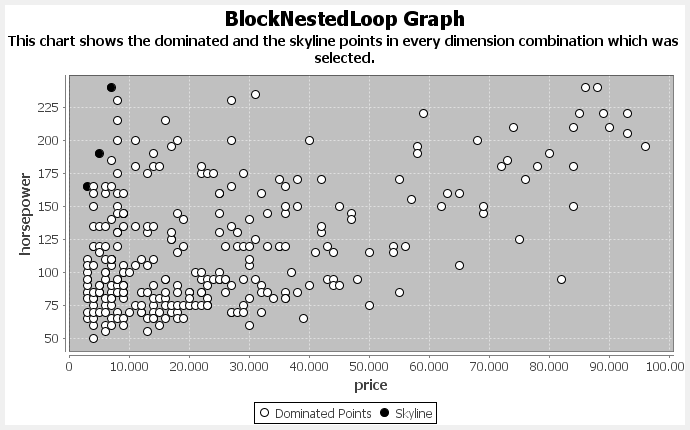
\includegraphics[scale=0.6]{skylineExample.png}
	\caption{Autobeispiel - Skyline mit den Dimensionen price und horsepower}
	\label{img:skylineExample}
\end{figure}


\begin{figure}[H]
	\centering
	\begin{adjustbox}{max size={\textwidth}{\textheight}}
    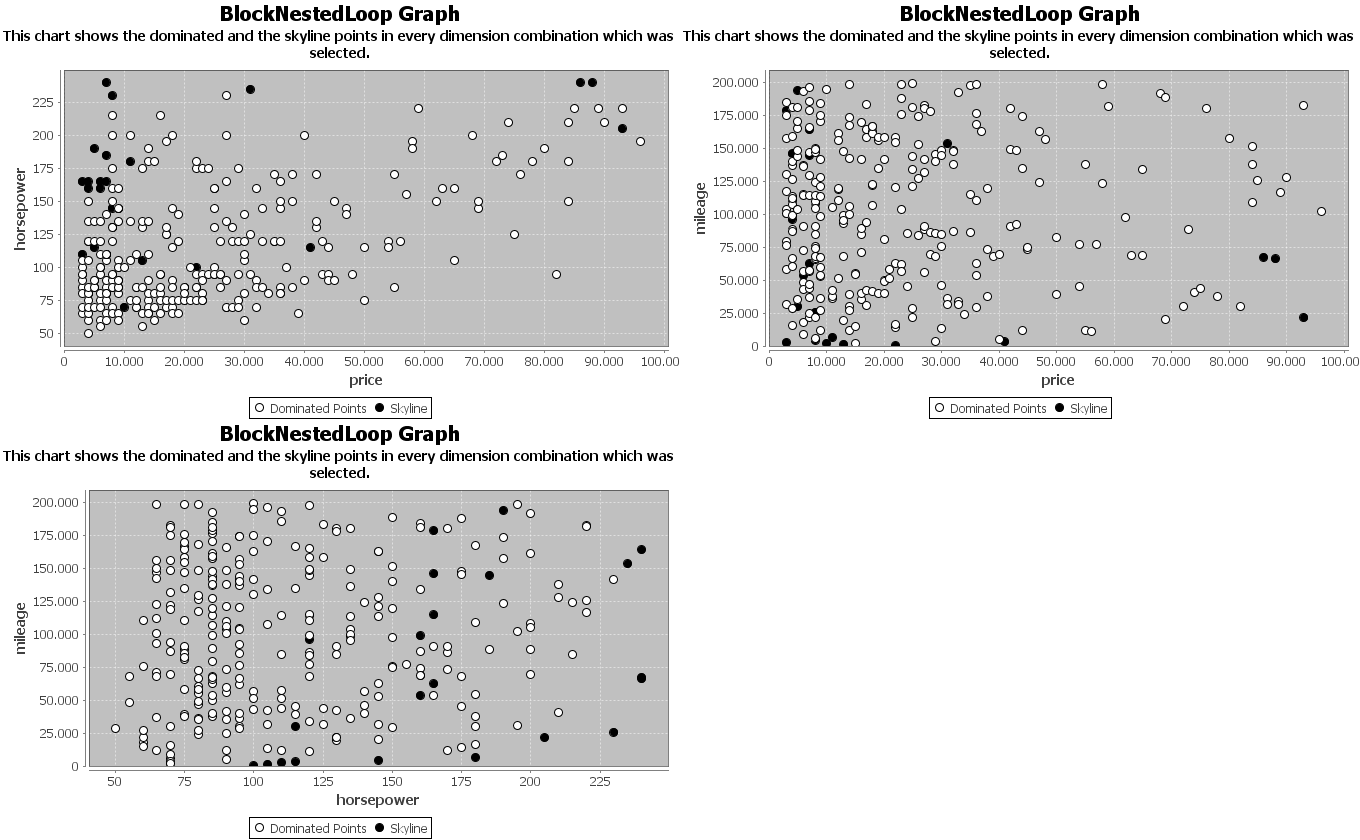
\includegraphics[]{skylineExampleMoreDimensions.png}
\end{adjustbox}
	\caption{Basketballspieler - Repräsentative Skyline mit Dimensionen Assists, Goals und Rebounds}
	\label{img:skylineExampleMoreDimensions}
\end{figure}

Aus diesen Erkenntnissen lässt sich schließen, dass bei zu vielen Dimensionen Skylines nicht mehr ihren Zweck erfüllen und repräsentative Skylines genutzt werden sollten. Auch wenn die entsprechenden Algorithmen für repräsentative Skylines meistens noch zusätzliche Rechenzeit mit sich bringen.
%% ==============================
\section{Repräsentative Skyline}
\label{ch:Grundlagen:sec:repSkyline}
%% ==============================
Eine repräsentative Skyline beinhaltet $k$ Datensätze der Skyline. Diese werden nach bestimmten Kriterien ausgewählt, wobei hier zwei hervorstechen: Signifikanz und Diversität.

Ein Datensatz ist signifikant, falls er einen bestimmten Threshold erfüllt, welcher meistens vom User festgelegt wird. Ein Threshold kann hierfür eine obere Grenze (Der Preis eines Autos sollte nicht 16000 \euro{} überschreiten) oder eine untere Grenze (Die PS Anzahl sollte nicht unter $100$ liegen) darstellen. 
Wie erwähnt ist es üblich diese Thresholds durch den User bestimmen zu lassen. Jedoch benutzen einige Ansätze (siehe \cite{36988}) vorhandene Daten von Usern, um passende Grenzen zu finden.

Wie der Name schon vermuten lässt, basiert Diversität auf der Unterschiedlichkeit von Datensätzen und soll so hoch wie möglich sein. Diese Unterschiedlichkeit wird oft durch Differenzen der Werte der Dimensionen oder der euklidischen Distanz zwischen den einzelnen Datensätzen berechnet. 
Aus diesen Gründen sind bei alleiniger Betrachtung des Diversitätskriteriums nur Datensätze in der repräsentativen Skyline, die weit voneinander entfernt sind. 

\begin{figure}[H]
	\centering
	\begin{tikzpicture}
	   \draw[style=help lines] (0,0) grid (9.9,9.9)
       [step=1cm]      (1,2) grid +(1,1);
       
        \foreach \x/\xtext in {1/1,2/2,3/3,4/4,5/5,6/6,7/7,8/8,9/9}
        \draw[shift={(\x,0)}] (0pt,2pt) -- (0pt,-2pt) node[below] {$\xtext$};

		 \foreach \y/\ytext in {1/1,2/2,3/3,4/4,5/5,6/6,7/7,8/8,9/9}
         \draw[shift={(0,\y)}] (2pt,0pt) -- (-2pt,0pt) node[left] {$\ytext$};        
        
        % 4x4 grid
        \draw (0, 0) grid (10, 0);
        % x-axis
        \draw [thick,->] (0, 0) -- (10.5, 0);
        % y-axis
        \draw [thick,->] (0, 0) -- (0, 10.5);
       	%a
        \draw [color=black, fill=black] (1, 9) circle (0.1);
        \node at (0.8, 8.5) {a};
        	%b
        \draw [color=black, fill=black] (2, 5) circle (0.1);
        \node at (1.8, 4.5) {b};
        	%c
        \draw [color=black, fill=black] (2.5, 4) circle (0.1);
        \node at (2.4, 3.5) {c};
        	%d
        \draw [color=black, fill=black] (3, 3) circle (0.1);
        \node at (2.8, 2.5) {d};
        	%e
        \draw [color=black, fill=black] (4, 2.5) circle (0.1);
        \node at (3.8, 2.2) {e};
        	%f
        \draw [color=black, fill=black] (8.5, 2) circle (0.1);
        \node at (8.4, 1.5) {f};
        	%g
        \draw [color=black, fill=black] (9, 1.5) circle (0.1);
        \node at (8.8, 1.2) {g};
        	%h
        \draw [color=black, fill=black] (9.5, 1) circle (0.1);
        \node at (9.4, 0.5) {h};
        % x-axis label
        \node at (10, -0.5) {x};
        % y-axis label
        \node at (0, 11) {y};
    \end{tikzpicture}
	\caption{Beispiel einer Skyline mit zwei Dimensionen}
	\label{img:diversitaetExample}
\end{figure}

Basierend auf dem Diversitätkriterium sind in Abbildung \ref{img:diversitaetExample} drei Punkte/Datensätze am besten geeignet für die repräsentative Skyline. Punkt $a$ repräsentiert sich am besten selber. Die Punkte $b,c,d,e$ werden am besten durch $c$ oder $d$ repräsentiert, da diese relativ mittig von dieser Menge liegen. Für die restlichen Punkte ist $g$ der geeignetste.
An diesem Beispiel ist zu erkennen, dass $k$ ein wichtiger Faktor ist, um eine hohe Repräsentationsgüte zu erreichen. Denn in diesem Beispiel ist der optimale Wert von $k$ drei und ein höherer Wert würde keinen Mehrwert bzw. keine deutlich höhere Repräsentationsgüte liefern da für $k=3$ jedes Cluster einen Repräsentant hat.
%% ==============================
\section{Präferenzen}
\label{ch:Grundlagen:sec:präferenzen}
%% ==============================
Anfragen an Suchmaschinen und Datenbanken haben oft das Problem, dass sie entweder einen \enquote{empty-result} Effekt (keine Ergebnisse) oder einen \enquote{flooding-effect} (zu viele Ergebnisse) liefern. Dies frustriert in vielen Fällen den User.
Um diesem Problem zu entgehen, wurde die Standard SQL-Sprache um Präferenzen erweitert. Die Idee dahinter ist, dass der User für ihn intuitive Präferenzen (z.B. ein Auto sollte nicht mehr als 16000 \euro{} kosten) erstellen kann. Anhand dieser Präferenzen werden daraufhin die besten Ergebnisse ausgesucht.

\begin{figure}[H]
\centering
\begin{tikzpicture}
    \node (SCORE) at (0,0) {SCORE};
    \node (EXPLICIT) at (-6,-1) {EXPLICIT};
    \node (LAYERED) at (-3,-2) {LAYERED};
    \node (CONTAINS) at (0,-2) {CONTAINS};
    \node (BETWEEN) at (3,-2) {BETWEEN};
    \node (POS/POS) at (-5,-3) {POS/POS};
    \node (POS/NEG) at (-1,-3) {POS/NEG};
    \node (AROUND) at (3,-3) {AROUND};
    \node (POS) at (-5,-4) {POS};
    \node (NEG) at (-1,-4) {NEG};
    \node (LOWEST) at (2,-4) {LOWEST};
    \node (HIGHEST) at (4,-4) {HIGHEST};
    \path [-] (EXPLICIT) edge node {} (POS/POS);
    \path [-] (POS/POS) edge node {} (POS);
    \path [-] (LAYERED) edge node {} (POS/POS);
    \path [-] (LAYERED) edge node {} (POS/NEG);
    \path [-] (POS/NEG) edge node {} (NEG);
    \path [-] (SCORE) edge node {} (LAYERED);
    \path [-] (SCORE) edge node {} (CONTAINS);
    \path [-] (SCORE) edge node {} (BETWEEN);
    \path [-] (BETWEEN) edge node {} (AROUND);
    \path [-] (AROUND) edge node {} (LOWEST);
    \path [-] (AROUND) edge node {} (HIGHEST);

\end{tikzpicture}
	\caption{Beispiel einer Skyline mit zwei Dimensionen}
	\label{img:preferences}
\end{figure} 

Abbildung \ref{img:preferences} gibt einen Überblick über alle Präferenzen in Preference-SQL. In dieser Arbeit werden nur die Basispräferenzen vorgestellt, die in KNIME implementiert wurden. Die BETWEEN Präferenz erlaubt es Werte einer Dimension in einem vom User bestimmten Intervall zu präferieren. Dagegen präferiert die AROUND Präferenz Datensätze, die nah an einem bestimmten Wert liegen. Mit der LAYERED Präferenz ist es möglich Werte einer Dimension nach Wichtigkeit zu sortieren. Für Autofarben könnte folgende Reihenfolge erstellt werden: grün > schwarz > others > rot. Diese Präferenz würde als erstes grüne, darauf folgend schwarze, danach alle anderen Autos und schlussendlich rote Autos präferieren.
Die LOWEST Präferenz (Werte sollen so klein wie möglich sein) und dessen Gegenstück HIGHEST sind auch in KNIME eingebunden worden, damit Standard Skylineabfragen wie Minimum und Maximum möglich sind.
Als Zusatz wurde eine BOOLEAN Präferenz hinzugefügt, die aus dem Preference-SQL Konzept von EXASolution entnommen wurde. (vgl. \cite{EXASolution}) Hier kann der User SQL Statements eingeben, die als boolische Ausdrücke gewertet werden. Alle Datensätze, die mit diesem Ausdruck übereinstimmen und dadurch $true$ ergeben, werden bevorzugt. Im Fall des Autobeispiels könnte dies wie folgt aussehen: $price < 16000$. Mit diesem Ausdruck würden alle Autos bevorzugt, die weniger als 16000 \euro{} kosten. Dabei macht es keinen Unterschied wie niedrig der Preis ist. Alle Autos unter 16000 \euro{} werden als gleich wichtig gesehen. 

Die einzelnen Basispräferenzen können weiterhin noch mit Pareto ('AND') oder Priorisierungs ('PRIOR TO') Präferenzen verknüpft werden. Pareto verknüpfte Präferenzen haben die gleiche Wichtigkeit, wobei dazu im Gegensatz Basispräferenzen mit einer Priorisierungsverknüpfung unterschiedliche Wichtigkeit besitzen. Hierbei ist die erst genannte Basispräferenz immer wichtiger als die zweite.  

Zusätzlich zu den Verknüpfungen oder auch komplexen Präferenzen genannt, gibt es das Best Matches Only Query Model. Durch dieses Model werden \enquote{emty-results} und \enquote{flooding-effects} gemieden, da es nur die besten Ergebnisse, die sich untereinander nicht dominieren, ausgibt. Durch die Dominanz werden schlechtere Datensätze nicht zur Ergebnismenge hinzugefügt und somit wird die Anzahl der Datensätze im Ergebnis reduziert. Falls keine Datensätze vorhanden sind, die die Präferenzen optimal berücksichtigen, werden die Nächstbesten als Ergebnis genommen. Dies führt dazu, dass die Ergebnisse immer die Präferenzen so gut wie möglich berücksichtigen und die Ergebnismenge nie leer sein kann.

In Abbildung \ref{img:prefSQLSyntax} ist die Syntax zu Preference-SQL zu sehen. Hier können nach der PREFERRING Klausel die Basispräferenzen mit genannten Verknüpfungen angegeben werden. Zusätzlich kann sortiert (GROUP BY) und eine Constraint (BUT ONLY),die den \enquote{flooding-effect} noch weiter reduziert, angegeben werden. Näheres dazu kann in den diesbezüglichen Paper (\cite{kiessling2011preference}, \cite{kiessling2002foundations} und \cite{kiessling2002preference}) gelesen werden.

\begin{figure}[H]
\centering
$\begin{matrix*}[l]
\text{SELECT} & \ldots & \text{<selection>} \\
\text{FROM} & \ldots & \text{<table\char`_reference>} \\
\text{WHERE} & \ldots & \text{<hard\char`_conditions>} \\
\hspace{10pt} \textbf{PREFERRING} & \ldots & \text{<soft\char`_conditions>} \\
\hspace{10pt} \textbf{GROUPING} & \ldots & \text{<attribute\char`_list>} \\
\hspace{10pt} \textbf{BUT ONLY} & \ldots & \text{<but\char`_only\char`_condition>} \\
\text{GROUP BY} & \ldots & \text{<attribute\char`_list>} \\
\text{HAVING} & \ldots & \text{<hard\char`_conditions>} \\
\text{ORDER BY} & \ldots & \text{<attribute\char`_list>} \\
\end{matrix*}$
	\caption{Syntax von Preference-SQL}
	\label{img:prefSQLSyntax}
\end{figure} 

Zum Schluss dieses Abschnittes wird die Syntax an einem Beispiel erklärt.
Angenommen es werden alle Autos mit der höchsten PS Leistung und dem geringsten Preis gesucht. Zusätzlich sollte die Kilometeranzahl um den Wert 100000 liegen, was jedoch nicht so wichtig ist wie der Preis.
Daraus entsteht folgender Query:
\begin{verbatim}
SELECT * 
FROM car 
PREFERRING (price LOWEST PRIOR TO mileage AROUND 100000) AND
horsepower HIGHEST
\end{verbatim}


Anhand dieses Queries kann mit dem Preference-SQL JDBC Präferenzabfragen an eine Datenbank geschickt werden.
%% ==============================
\section{KNIME}
\label{ch:Grundlagen:sec:knime}
%% ==============================
KNIME oder der Konstanz Information Miner ist eine modulare Umgebung, die einen einfachen visuellen Zusammenbau und eine interaktive Ausführung von einer Data Pipeline ermöglicht. Es wird damit geworben, dass es \enquote{easy and intuitive to use} ist und \enquote{enables the user to visually explore the results} \cite[p. 2]{BCDG+07}. 

Der Konstanz Information Miner ist in Java geschrieben und dessen graphischer Workflow Editor ist als ein Eclipse Plug-in implementiert worden. Mit einer offenen API und einem Datenabstraktions Framework wird dem User erlaubt schnell Nodes zu implementieren und diese einem Workflow hinzuzufügen.

Die Architektur von KNIME unterliegt drei Prinzipien. Einem visuellen und interaktivem Framework, welches dem User ermöglicht durch einfaches Drag \& Drop Datenflüsse zu kombinieren und somit verschiedene Node Outputs als Input für andere Nodes verwenden zu können. Modularität sorgt dafür, dass alles unabhängig voneinander funktioniert. Seien es Prozesseinheiten oder Datencontainer. Dies ermöglicht eine unabhängige Implementierung von verschiedenen Algorithmen. Das letzte Prinzip ist die einfache Erweiterbarkeit. Entwickler können auf die öffentliche API zugreifen und durch das Eclipse Plug-In-Schema ohne Probleme neue Nodes entwickeln. (vgl. \cite{BCDG+07})

KNIME ermöglicht neue Algorithmen oder Visualisierungen als Nodes in KNIME zu integrieren. Nodes besitzen In- und Output Ports, die den Ein- und Ausgaben des darunter liegenden Algorithmus entsprechen. Nodes bestehen hauptsächlich aus drei Teilen: NodeModel, NodeDialog und NodeView. Das NodeModel ist dafür zuständig, dass der Algorithmus ausgeführt wird und wichtige Einstellungen gespeichert werden. Es testet, ob mit den Eingabe des Nodes der Algorithmus korrekt durchgeführt werden kann und gibt die Ergebnisse des Algorithmus aus. 
Der NodeDialog ermöglicht es dem User bestimmte Einstellungen für den Algorithmus vorzunehmen. Hierbei kann eine eigene GUI geschrieben werden oder die von KNIME vorliegenden Standardkomponenten verwendet werden. Die Kommunikation zwischen dem NodeModel und dem NodeView erfolgt durch eine Speicherung von SettingsModels in ein NodeSettings Objekt, welches von beiden Klassen geladen und gespeichert werden kann. 
Das NodeView Objekt erstellt eine graphische Darstellung der Ergebnisse des Algorithmus. Dies kann ein Histogramm, Koordinatensystem oder ähnliches sein. Die Daten für diesen View müssen vom NodeModel in einer Datei gespeichert werden, um diesen View beim Wiederöffnen von KNIME neu zu erstellen. Dies ist erforderlich, sodass zu jeder Zeit der View betrachtet werden kann und dies nicht nur nach Ausführung des Nodes möglich ist.

Workflows sind Graphen in KNIME, genau genommen gerichtete azyklische Graphen. Der dazugehörige WorkflowManager verhilft es dem User neue Nodes zum Workflow und Verbindungen zwischen den Nodes hinzuzufügen.

\begin{figure}[H]
	\centering
	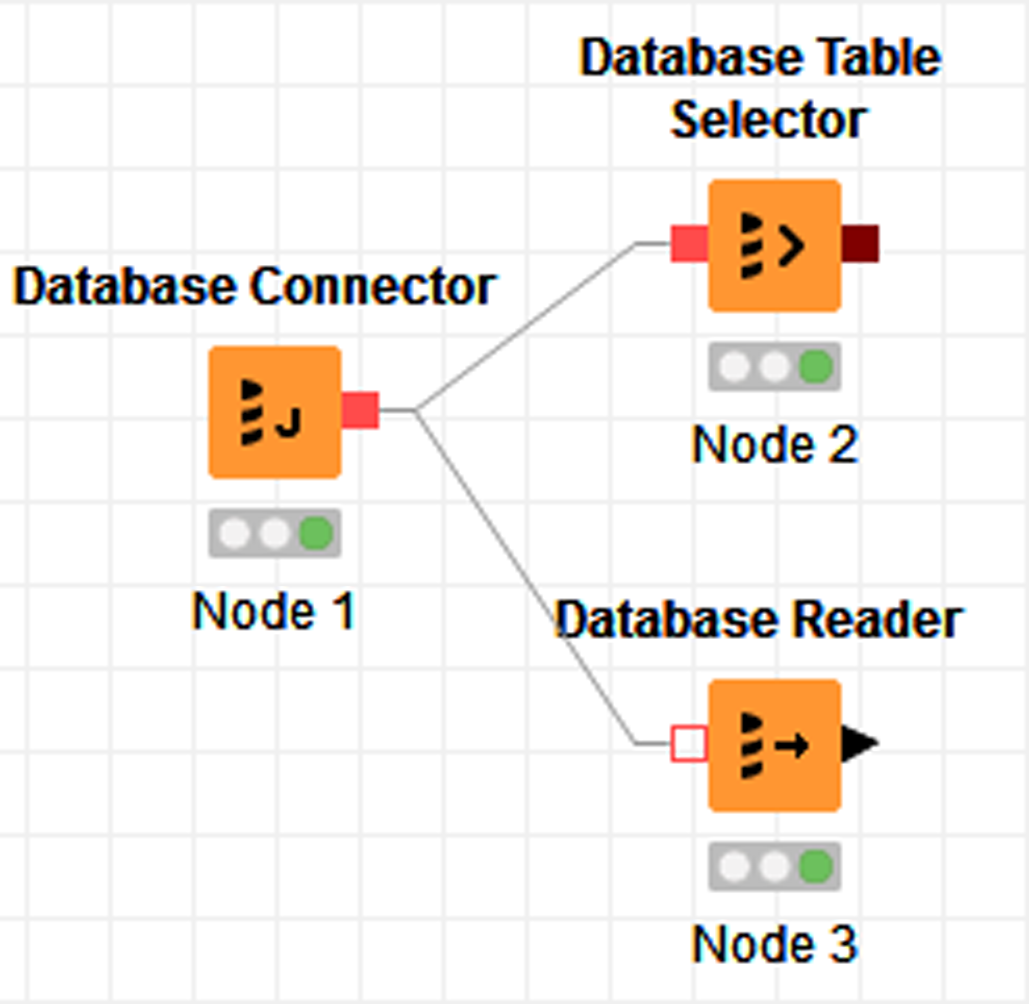
\includegraphics[scale=0.8]{workflowExample.png}
	\caption{Beispiel Workflow in KNIME}
	\label{img:workflowExample}
\end{figure}

In der Abbildung \ref{img:workflowExample} ist ein Beispiel eines Workflows zu erkennen. Mit dem \textit{SQLite Connector} Node kann eine SQLite Datenbankdatei auf dem Rechner ausgewählt werden und eine Verbindung zu dieser Datenbank aufgebaut werden. Diese Verbindung wird an die anderen Nodes als Input geschickt. Für den \textit{Database Table Selector} als auch den \textit{Database Reader} Node muss eine SQL-Query im NodeDialog eingegeben werden. Der \textit{Database Table Selector} gibt eine Datenbankverbindung mit dem entsprechenden Query zurück. Im Gegensatz dazu gibt der \textit{Database Reader} Node eine Tabelle zurück, die durch die SQL Abfrage an die Datenbank entsteht. Diese Datentabellen werden in KNIME BufferedDataTables genannt. 

Da nun Preference-SQL und KNIME genauer erklärt wurden, können im nächsten Kapitel die implementieren Algorithmen vorgestellt werden.
%% ==============================
%%% End: 